\normalfalse \difficiletrue \tdifficilefalse
\correctiontrue
%\UPSTIidClasse{12} % 11 sup, 12 spé
%\newcommand{\UPSTIidClasse}{12}

\exer{Mouvement RT -- RSG  $\star\star$ \label{C1:05:09}}
\setcounter{question}{0}\UPSTIcompetence[2]{B2-14}
\UPSTIcompetence[2]{C1-05}
\index{Compétence B2-14}
\index{Compétence C1-05}
\index{Principe fondamental de la dynamique}
\index{PFD}
\index{Mécanisme à 1 rotations, 1 translation et RSG}
\index{Culbuto}
\ifcorrection
\else
\marginnote{\textbf{Pas de corrigé pour cet exercice.}}
\fi

\ifprof
\else
Soit le mécanisme suivant. On a $\vect{IA}=R\vect{j_0}$ et $\vect{AB}=\ell_2\vect{i_1}$. De plus $R=\SI{15}{mm}$.
On fait l'hypothèse de roulement sans glissement au point $I$. De plus :
\begin{itemize}
\item $G_1$ désigne le centre d'inertie de \textbf{1} tel que $\vect{AG_1}=-\ell\vect{i_1}$, on note $m_1$ la masse de \textbf{1};% et $\inertie{G_1}{1}=\matinertie{A_1}{B_1}{C_1}{0}{0}{0}{\bas{1}}$; 
\item $G_2=B$ désigne le centre d'inertie de \textbf{2}, on note $m_2$ la masse de \textbf{2}.% et $\inertie{G_2}{2}=\matinertie{A_2}{B_2}{C_2}{0}{0}{0}{\bas{2}}$.
\end{itemize}
Un ressort exerce une action mécanique entre les points $A$ et $B$. 
\begin{center}
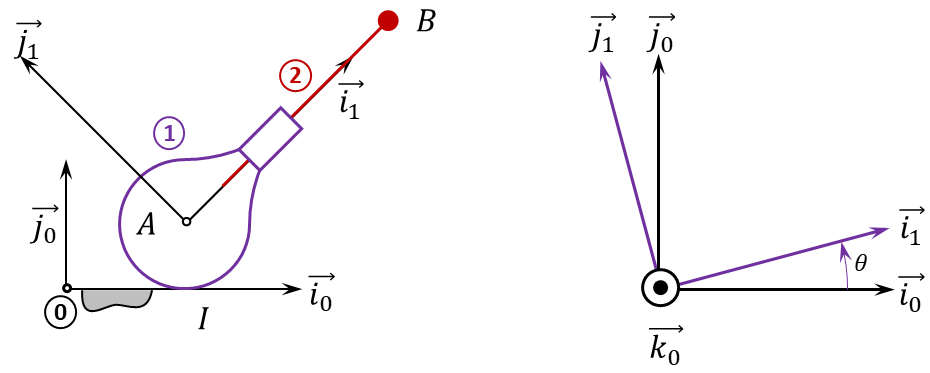
\includegraphics[width=\linewidth]{09_RT_RSG_01}
\end{center}
\fi

\question{Réaliser le graphe d'analyse en faisant apparaître l'ensemble des actions mécaniques.}
\ifprof
\begin{center}
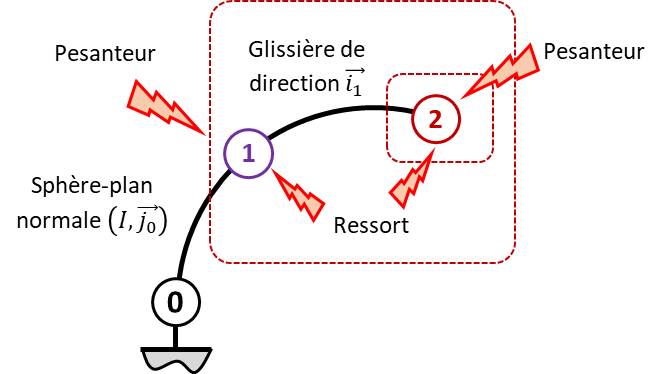
\includegraphics[width=.7\linewidth]{09_RT_RSG_cor_01}
\end{center}

\else
\fi

\question{Proposer une démarche permettant de déterminer les loi de mouvement de \textbf{1} et de \textbf{2} par rapport à~$\rep{0}$.}
\ifprof
Le système posède deux mobilités : 
\begin{itemize}
\item translation de 1 par rapport à 2 ($\lambda$);
\item rotation de l'ensemble \{1+2\} autour du point $I$ (le roulement sans glissement permet d'écrire une relation entre la rotation de paramètre $\theta$ et le déplacement suivant $\vi{0}$.
\end{itemize}

On en déduit la stratégie suivante : 
\begin{itemize}
\item on isole 2 et on réalise un théorème de la résultante dynamique en projection suivant $\vi{1}$. BAME : 
$\torseurstat{T}{1}{2}$, $\torseurstat{T}{1_{\text{ressort}}}{2}$ ($\vectf{1}{2}\cdot \vi{1}= 0$ et 
$\vectf{1_{\text{ressort}}}{2}\cdot \vi{1}= 0$)
$\torseurstat{T}{\text{Pesanteur}}{2}$.
\item on isole \{1+2\} et on réalise un théorème du moment dynamique en $I$ en projection suivant $\vk{0}$. BAME : 
$\torseurstat{T}{0}{1}$ ($\vectm{I}{0}{1}\cdot \vk{0}= 0$), 
$\torseurstat{T}{\text{Pesanteur}}{1}$ et $\torseurstat{T}{\text{Pesanteur}}{2}$.

\end{itemize}
\else
\fi

\ifcolle
\question{Déterminer les lois de mouvement.}
\else
\fi

\ifprof
\else
\begin{flushright}
\footnotesize{Corrigé  voir \ref{C1:05:09}.}
\end{flushright}%
\fi